\section{Introduction}
Continual learning aims to continually train models with new tasks without forgetting previously learned tasks \cite{ke2022continual,De}. It  has become a promising direction for NLP models to incrementally learn new tasks/domains/classes as humans do \cite{ke2022continual}. A typical scenario aims to enable NLP models to solve various tasks in an incremental manner, namely the task-incremental continual learning scenario, which is our study setting in this paper. A salient challenge for continual learning is that continually learned models usually suffer from cartographic forgetting (CF), i.e. the performance on previously learned tasks decreases after training on the new one \cite{lopez2017gradient}.

\begin{figure}
    \centering
    
\includegraphics[width=0.8\hsize]{fig1.png}
    \caption{Illustration of representations after contrastive continual learning on a task before and after learning a new task.  }
    \label{illu}
    \vspace{-5mm}
\end{figure}

%  Unlike the general training setup, where the training data for different tasks are simultaneously available, the data are fed to the model in a stream for continual training. 

 Various training strategies have been proposed to mitigate CF \cite{li2017learning,kirkpatrick2017overcoming,lopez2017gradient}. Under the fixed model structure, regularization-based methods design regularization terms to control the shift of representations learned from previous tasks \cite{li2017learning,kirkpatrick2017overcoming,aljundi2018memory}. Rehearsal-based methods  save the data samples from previous tasks into a memory buffer and re-train the model to recover knowledge during training on the current task  \cite{riemer2019learning,lopez2017gradient,de2019episodic}.
 However, most continual learning methods are designed to recover the learned knowledge or mitigate the representation of forgetting. 
 
% The methods of embedding networks, which directly learn the representations on the feature space, can mitigate the above issue \cite{chopra2005learning,yu2020semantic,luo2022mere}. 
Seldom considers adapting the classification criterion for the newly learned representations.
For example,  in supervised contrastive learning, the contrastive objective is designed to pull the data representations with the same labels together and push representations with different labels away \cite{Chen2020,gao-etal-2021-simcse,zhang-etal-2021-pairwise,neelakantan2022text,zhaoconsistent}. Representations of the training samples can be saved as a classification criterion, after which an instance-based method such as  a k Nearest Neighbor (kNN) module  can be leveraged for inference \cite{kassnerbert,khandelwal2020nearest}. After learning the new task, we can feed the saved sample into models for new classification criteria and mitigate the problem of CF. For example in Figure 1, although the representations have decayed for learning the new task, the saved samples adapt to serve as the classification criterion in kNN modules.

% It has been proved that such supervised contrastive learning methods in feature space have stronger robustness and generalization ability compared with standard cross-entropy-based methods \cite{khosla2020supervised,gunel2020supervised,luo2022mere,cha2021co2l}.  


Inspired by the above motivation, we investigate the use of supervised contrastive learning for task-incremental continual learning (SCCL). After supervised contrastive learning on each task, we use a K-means module to select several samples and save them into a memory buffer while maintaining the  learned representation distribution.  In addition, to mitigate the representation drift when training the model for new tasks, we use an instance-wise relation distillation (IRD) term \cite{fang2020seed,cha2021co2l} and a memory replay module \cite{de2019episodic} to maintain the learned knowledge.
During inference, the saved samples are fed into the trained model to obtain updated representations and a kNN module is used for classification.
% For example,  in supervised contrastive learning, the contrastive objective is designed to pull the data representations with the same labels together and push  representations with different labels away \cite{Chen2020,gao-etal-2021-simcse,zhang-etal-2021-pairwise,neelakantan2022text}. Representations of the training samples can be saved as a classification criterion, after which an instance-based method such as  a k Nearest Neighbor (kNN) module  can be leveraged for inference \cite{kassnerbert,khandelwal2020nearest}.  It has been proved that such supervised contrastive learning methods in feature space have stronger robustness and generalization ability compared with standard cross-entropy-based methods \cite{khosla2020supervised,gunel2020supervised,luo2022mere,cha2021co2l}.  




Experimental results show that our proposed model can achieve state-of-the-art performance compared with standard cross-entropy-based (CE) baselines. We additionally extend different continual learning strategies \cite{kirkpatrick2017overcoming,aljundi2018memory,li2017learning} to the supervised  contrastive continual learning framework, which gives stronger results than corresponding CE-based methods, showing the advantage of contrastive learning with a kNN classifier in continual learning scenarios. We further analyze  the effectiveness of each module in our paper through ablation studies.  To our knowledge, we are the first to propose a supervised contrastive learning framework for task-incremental continual learning, without any augmented parameters. The code will be released when accepted.



\begin{figure*}
    \centering
    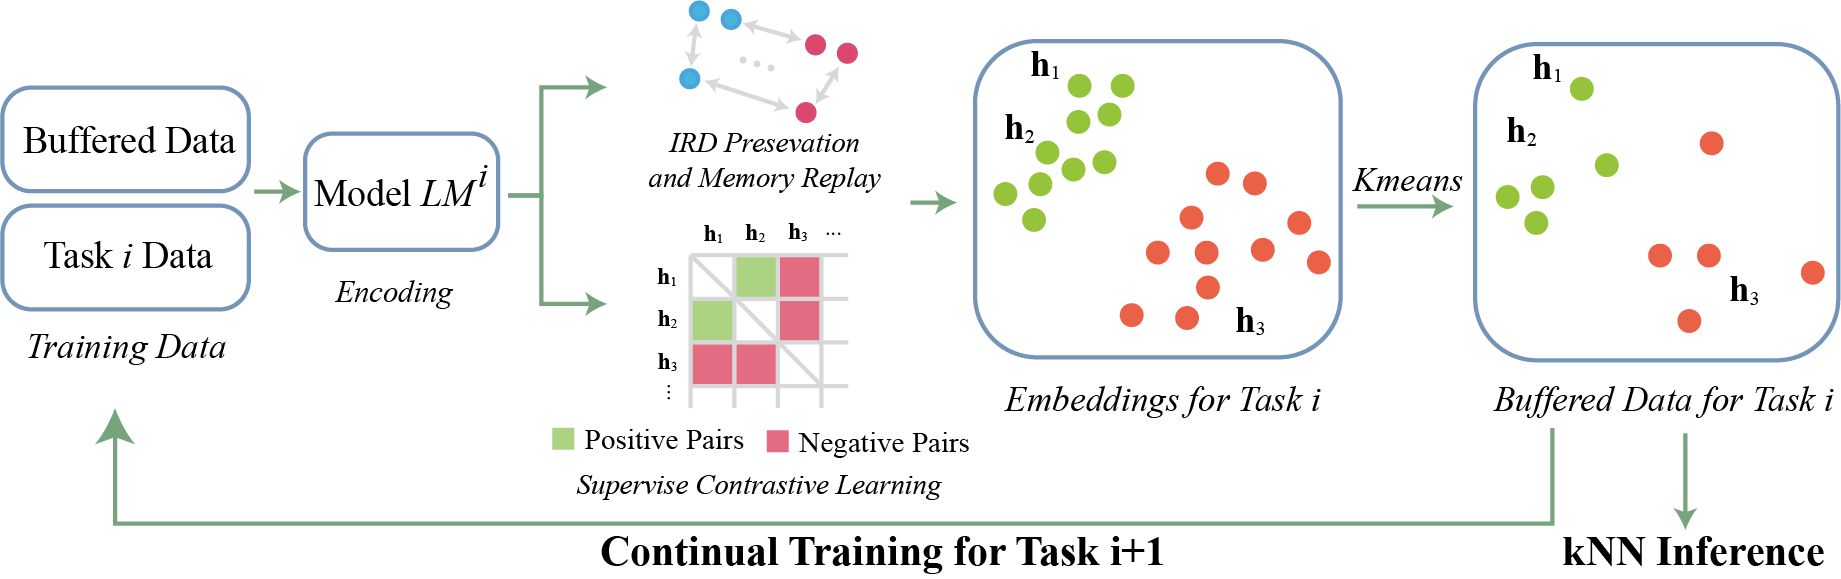
\includegraphics[width=0.9\hsize]{SCOCL.png}
    \caption{The model framework of SCCL contains four main modules: (1) the supervised contrastive learning for each task; (2) the explicit control of catastrophic forgetting with IRD knowledge distillation and memory replay; (3) the selection of learned representations; (4) a kNN inference module. }
    \label{framework}
        \vspace{-4mm}
\end{figure*}